\documentclass[preview]{standalone}

\usepackage{amsmath}
\usepackage{amssymb}
\usepackage{tikz}
\usepackage{stellar}
\usepackage{definitions}

\begin{document}

\id{matrix-polynomials-jordan-form}
\genpage

\section{Similarity and polynomial evaluation}

\begin{snippetproposition}{matrix-polynomial-similarity-compatibility}{Polynomial evaluation commutes with similarity}
    Let \(A,B\in\matrices_n(K)\), let \(f\in K[X]\), and suppose
    \[
        B=P^{-1}AP.
    \]
    Then
    \[
        f(B)=P^{-1}f(A)P.
    \]
    In particular, if \(J(A)=P^{-1}AP\) is a Jordan form of \(A\), then
    the \matrixpolynomial \(f(A)\) is similar to \(f(J(A))\).
\end{snippetproposition}

\begin{snippetproof}{matrix-polynomial-similarity-compatibility-proof}{matrix-polynomial-similarity-compatibility}{Polynomial evaluation commutes with similarity}
    For every \(m\geq0\),
    \[
        B^m=P^{-1}A^mP.
    \]
    If \(f=\sum_m c_mX^m\), then
    \[
        f(B)
        =
        \sum_m c_mB^m
        =
        P^{-1}\left(\sum_m c_mA^m\right)P
        =
        P^{-1}f(A)P.
    \]
\end{snippetproof}

\begin{snippetnote}{matrix-polynomial-jordan-form-warning}{Evaluating a Jordan form need not produce a Jordan form}
    Although \(f(A)\) is similar to \(f(J(A))\), the matrix
    \(f(J(A))\) need not itself be in Jordan canonical form. Its blocks
    may have to be reduced further, and distinct eigenvalues of \(A\)
    may be sent to the same eigenvalue by \(f\).
\end{snippetnote}

\section{When block sizes are preserved}

\begin{snippetproposition}{matrix-polynomial-jordan-block-derivative}{A nonzero derivative preserves a Jordan-block size}
    Let \(f\in K[X]\), \(a\in K\), and \(m\geq1\). If
    \[
        f'(a)\neq0,
    \]
    then
    \[
        f(J_m(a))
        \sim
        J_m(f(a)).
    \]
\end{snippetproposition}

\begin{snippetproof}{matrix-polynomial-jordan-block-derivative-proof}{matrix-polynomial-jordan-block-derivative}{A nonzero derivative preserves a Jordan-block size}
    Write
    \[
        f(X)-f(a)=(X-a)q(X).
    \]
    Then \(q(a)=f'(a)\neq0\). With \(J_m(a)=aI_m+N_m\),
    \[
        f(J_m(a))-f(a)I_m
        =
        N_mq(J_m(a)).
    \]
    The matrix \(q(J_m(a))\) is a polynomial in \(N_m\) with nonzero
    constant term \(q(a)\), so it is invertible; it also commutes with
    \(N_m\). Consequently, for every \(k\geq0\),
    \[
        \mrank\left(
            \big(f(J_m(a))-f(a)I_m\big)^k
        \right)
        =
        \mrank(N_m^k).
    \]
    These ranks characterize a single nilpotent Jordan block of size
    \(m\). Hence \(f(J_m(a))\) is similar to \(J_m(f(a))\).
\end{snippetproof}

\begin{snippetnote}{matrix-polynomial-vanishing-order-block-splitting}{What happens when the derivative vanishes}
    More generally, if \(s\geq1\) is the multiplicity of \(a\) as a
    root of \(f(X)-f(a)\), then
    \[
        f(J_m(a))-f(a)I_m
        =
        N_m^sQ(N_m)
    \]
    for an invertible matrix \(Q(N_m)\). Thus its ranks are those of
    the powers \(N_m^{sk}\). When \(s>1\), the original Jordan block can
    split into several smaller blocks.
\end{snippetnote}

\section{Example}

\begin{snippetexample}{matrix-polynomial-a-plus-a-squared-example}{The polynomial \(f(X)=X+X^2\)}
    Let \(K\) have characteristic \(0\), and suppose
    \[
        J(A)=J_3(0)\oplus J_2(3)\oplus J_1(3).
    \]
    Put
    \[
        B=A+A^2=f(A),
        \qquad
        f(X)=X+X^2.
    \]
    Since
    \[
        f(0)=0,
        \qquad
        f(3)=12,
    \]
    the characteristic polynomial is
    \[
        \chi_B=X^3(X-12)^3.
    \]
    Moreover,
    \[
        f'(X)=1+2X,
        \qquad
        f'(0)=1\neq0,
        \qquad
        f'(3)=7\neq0.
    \]
    The Jordan-block sizes are therefore preserved:
    \[
        J(B)=J_3(0)\oplus J_2(12)\oplus J_1(12).
    \]
    It follows that
    \[
        \mu_B=X^3(X-12)^2.
    \]

    For the invariant factors, right-align the single \(0\)-primary
    block of size \(3\) with the \(12\)-primary blocks of sizes \(1\)
    and \(2\). This gives
    \[
        V_B
        \moduleisomorphic
        K[X]/(X-12)
        \oplus
        K[X]/\big(X^3(X-12)^2\big),
    \]
    so the invariant factors are
    \[
        X-12,
        \qquad
        X^3(X-12)^2.
    \]

    The original column picture is:
    \[
        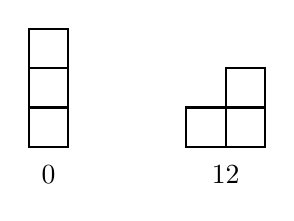
\begin{tikzpicture}[scale=0.5]
            \foreach \x/\h in {0/3} {
                \foreach \y in {1,...,\h} {
                    \draw[thick] (\x,\y-1) rectangle (\x+1,\y);
                }
            }
            \node at (0.5,-0.7) {\(0\)};

            \begin{scope}[xshift=4cm]
                \foreach \x/\h in {0/1,1/2} {
                    \foreach \y in {1,...,\h} {
                        \draw[thick] (\x,\y-1) rectangle (\x+1,\y);
                    }
                }
                \node at (1,-0.7) {\(12\)};
            \end{scope}
        \end{tikzpicture}
    \]
\end{snippetexample}

\end{document}
